\section{Exercises and Solutions of \texorpdfstring{\cite{gf}}{Lg}}

\subsection{June 11-13 Local structure of fractals(5)}
\subsubsection{Exercises and Solutions}
\begin{customexercise}{5.2}
    Let $f: \mathbb{R} \rightarrow \mathbb{R}$ be a continuously differentiable function such that $0<c_{1} \leq f^{\prime}(x) \leq c_{2}$ for all $x .$ Show that if $F$ is an $s$-set in $\mathbb{R}$, then $\underline{D}^{s}(f(F), f(x))=\underline{D}^{s}(F, x)$ for all $x$ in $\mathbb{R}$, with a similar result for upper densities.    
\end{customexercise}

\begin{customsol}{5.2}

\end{customsol}

\begin{customexercise}{5.8}
    Let $F_{1}, F_{2}, \ldots$ be 1-sets in the plane such that $F=\bigcup_{k=1}^{\infty} F_{k}$ is a 1-set. Show that if $F_{k}$ is regular for all $k$, then $F$ is regular, and if $F_{k}$ is irregular for all $k$, then $F$ is irregular.
\end{customexercise}

\begin{customsol}{5.8}
    
\end{customsol}

\newpage

\subsection{June 8 Hausdorff and packing measures and dimensions(3)}
\subsubsection{Exercises and Solutions}
\begin{customexercise}{3.7}
    Let $f:[0,1] \rightarrow \mathbb{R}$ be a Lipschitz function. Writing $\operatorname{graph} f=\{(x, f(x)): 0 \leq x \leq 1\}$, show that $\operatorname{dim}_{\mathrm{H}}$ graph $f=1 .$ Note, in
particular, that this is true if $f$ is continuously differentiable, see Exercise \ref{1.13}.
\end{customexercise}
\begin{customsol}{3.7}
   Let $g(x)=(x, f(x))$ where $g:[0,1] \rightarrow \operatorname{graph} f$. Then $g$ is bi-Lipschitz, since:
$$
|g(x)-g(y)|^{2}=|x-y|^{2}+|f(x)-f(y)|^{2}
$$
Then,
$$
|x-y|^{2} \leq|g(x)-g(y)|^{2} \leq|x-y|^{2}+c^{2}|x-y|^{2}=\left(1+c^{2}\right)|x-y|^{2}
$$
since $|f(x)-f(y)| \leq c|x-y|$ for some $c>0$. Thus by taking the square root, $g$ is bi-Lipschitz. Therefore, by Proposition \ref{H-under-L} b., 
$$\operatorname{dim}_{\mathrm{H}} \operatorname{graph} f = \operatorname{dim}_{\mathrm{H}} g([0,1]) = \operatorname{dim}_{\mathrm{H}}([0,1]) = 1$$
\end{customsol}

\textbf{Note: }If $f$ is Lipschitz(or $f$ is continuously differentiable), then graph $f$ is bi-Lipschitz. 


\begin{customexercise}{}
    Prove Proposition \ref{H-under-L}:
    \begin{enumerate}[(a)]
        \item Let $F \subset \mathbb{R}^{n}$ and suppose that $f: F \rightarrow \mathbb{R}^{m}$ satisfies the Hölder condition
$$
|f(x)-f(y)| \leq c|x-y|^{\alpha} \quad(x, y \in F) .
$$
Then $\operatorname{dim}_{\mathrm{H}} f(F) \leq(1 / \alpha) \operatorname{dim}_{\mathrm{H}} F .$ In particular, if $f$ is a Lipschitz
mapping, that is, if $\alpha=1$, then $\operatorname{dim}_{H} f(F) \leq \operatorname{dim}_{H} F$.
\item If $f: F \rightarrow \mathbb{R}^{m}$ is a bi-Lipschitz transformation, that is,
$$
c_{1}|x-y| \leq|f(x)-f(y)| \leq c|x-y| \quad(x, y \in F),
$$
where $0<c_{1} \leq c<\infty$, then $\operatorname{dim}_{\mathrm{H}} f(F)=\operatorname{dim}_{\mathrm{H}} F$.
    \end{enumerate}
\end{customexercise}

\begin{customsol}{} $ $
    \begin{enumerate}[(a)]
        \item If $s>\operatorname{dim}_{\mathrm{H}} F$, then by Proposition 3.1 $\mathcal{H}^{s / \alpha}(f(F)) \leq c^{s / \alpha} \mathcal{H}^{s}(F)=0$,
        implying that $\operatorname{dim}_{\mathrm{H}} f(F) \leq s / \alpha$ for all $s>\operatorname{dim}_{\mathrm{H}} F$. The conclusion for
        Lipschitz mappings is immediate on taking $\alpha=1$.
        \item For the bi-Lipschitz case, just as in Proposition $2.5$ for box dimension, applying the Lipschitz result to $f^{-1}: f(F) \rightarrow F$ yields the reverse inequality $\operatorname{dim}_{\mathrm{H}} F \leq \operatorname{dim}_{\mathrm{H}} f(F)$.
    \end{enumerate}
\end{customsol}

\newpage

\subsection{June 4-6 Box-counting dimension(2)}
\subsubsection{Exercises and Solutions}

\begin{customexercise}{2.1}
    Verify directly from the definitions that Equivalent definitions \ref{bcd-def}(ii) and (iv) give the same values for box dimension.
\end{customexercise}

\begin{customsol}{2.1}
    Let $F$ be a subset of $\mathbb{R}^{n}$, let $N_{\delta}(F)$ denote the smallest number of closed balls of radius $\delta$ that cover $F$ and let $N_{\delta}^{\prime}(F)$ denote the number of $\delta$-mesh cubes that intersect $F$. 
    Consider that the closed ball of radius $\delta\sqrt{n}$ will definitely contains the $\delta$-mesh cube when centers are the same. On the other hand, any closed ball of radius $\delta$ is intersect(and contained if center of the ball is the center of all cubes) at most $4^n$ $\delta$-mesh cubes. Thus, 
    $$
    N_{\delta \sqrt{n}}(F) \leq N_{\delta}^{\prime}(F) \leq 4^{n} N_{\delta}(F)
    $$
    Combining this inequality and dividing by $-\log \delta$,
$$
\frac{\log N_{\delta \sqrt{n}}(F)}{-\log (\delta \sqrt{n})+\log \sqrt{n}} \leq \frac{\log N_{\delta}^{\prime}(F)}{-\log \delta} \leq \frac{\log 4^{n}+\log N_{\delta}(F)}{-\log \delta}
$$
so taking lower limits as $\delta \rightarrow 0$ where $\delta\sqrt{n}\rightarrow 0 $ as well,
$$
\lowlim _{\delta \rightarrow 0} \frac{\log N_{\delta}(F)}{-\log \delta} \leq \lowlim _{\delta \rightarrow 0} \frac{\log N_{\delta}^{\prime}(F)}{-\log \delta} \leq \lowlim _{\delta \rightarrow 0} \frac{\log N_{\delta}(F)}{-\log \delta},
$$
with the other terms disappearing in the limit. Thus, the definition of lower box dimension is the same working with either $N_{\delta}(F)$ or $N_{\delta}^{\prime}(F)$. Taking upper limits, we get a similar conclusion for upper box dimension.
\end{customsol}


\begin{customexercise}{2.2}
    Generalise Proposition \ref{prop2.5} by showing that if $f: F \rightarrow \mathbb{R}^{n}$ satisfies the Hölder condition $|f(x)-f(y)| \leq c|x-y|^{\alpha}$ where $c>0$ and $0<\alpha \leq 1$, then $\underline{\operatorname{dim}_{B}} f(F) \leq(1 / \alpha) \underline{\operatorname{dim}}_{\mathrm{B}} F$ and $\overline{\operatorname{dim}}_{\mathrm{B}} f(F) \leq(1 / \alpha) \overline{\operatorname{dim}}_{\mathrm{B}} F$.
\end{customexercise}

\begin{customsol}{2.2}
    Note that if $\{U_i\}$ is a $\delta$-cover of $F$, then so $\{U_i\cap F\}$. Then, as
    $$
    |f(U_i\cap F)|\leq c|U_i\cap F|^\alpha\leq c|U_i|^\alpha\leq c\delta^\alpha
    $$
    (this can be understood as taking $x, y\in U_i\cap F$ or $x, y\in U_i$ where $|x-y|<\delta$ by construction)
    s.t. $\{f(U_i\cap F)\}$ is a $c\delta^\alpha$ cover of $f(F)$, and hence $N_{c\delta^\alpha}(f(F)) \leq N_\delta(F), \forall \delta>0$(consider $f$ is injective, or, we may have a better cover when considered overall for the image). Thus,
    $$
    \begin{aligned} \underline{\operatorname{dim}}_{B} f(F) &=\varliminf_{c \delta^{\alpha} \rightarrow 0} \frac{\log N_{c \delta^{\alpha}}(f(F))}{-\log c \delta^{\alpha}} \\
        &\leq \varliminf_{\delta \rightarrow 0} \frac{\log N_{\delta}(F)}{-\alpha \log \delta-\log c} \\ &=\frac{1}{\alpha} \varliminf_{\delta \rightarrow 0} \frac{\log N_{\delta}(F)}{-\log \delta}\\
        &=\frac{1}{\alpha} \underline{\operatorname{dim}}_{B} F \end{aligned}
    $$
    and same process can be applied for upper box-counting dimension. 
\end{customsol}


\begin{customexercise}{2.4}\label{calculation}
    Verify that the Cantor dust depicted in Figure \ref{fig:cantordust}, has box dimension 1 (take $E_{0}$ to have side length 1).
    \begin{figure}[H]
        \centering
        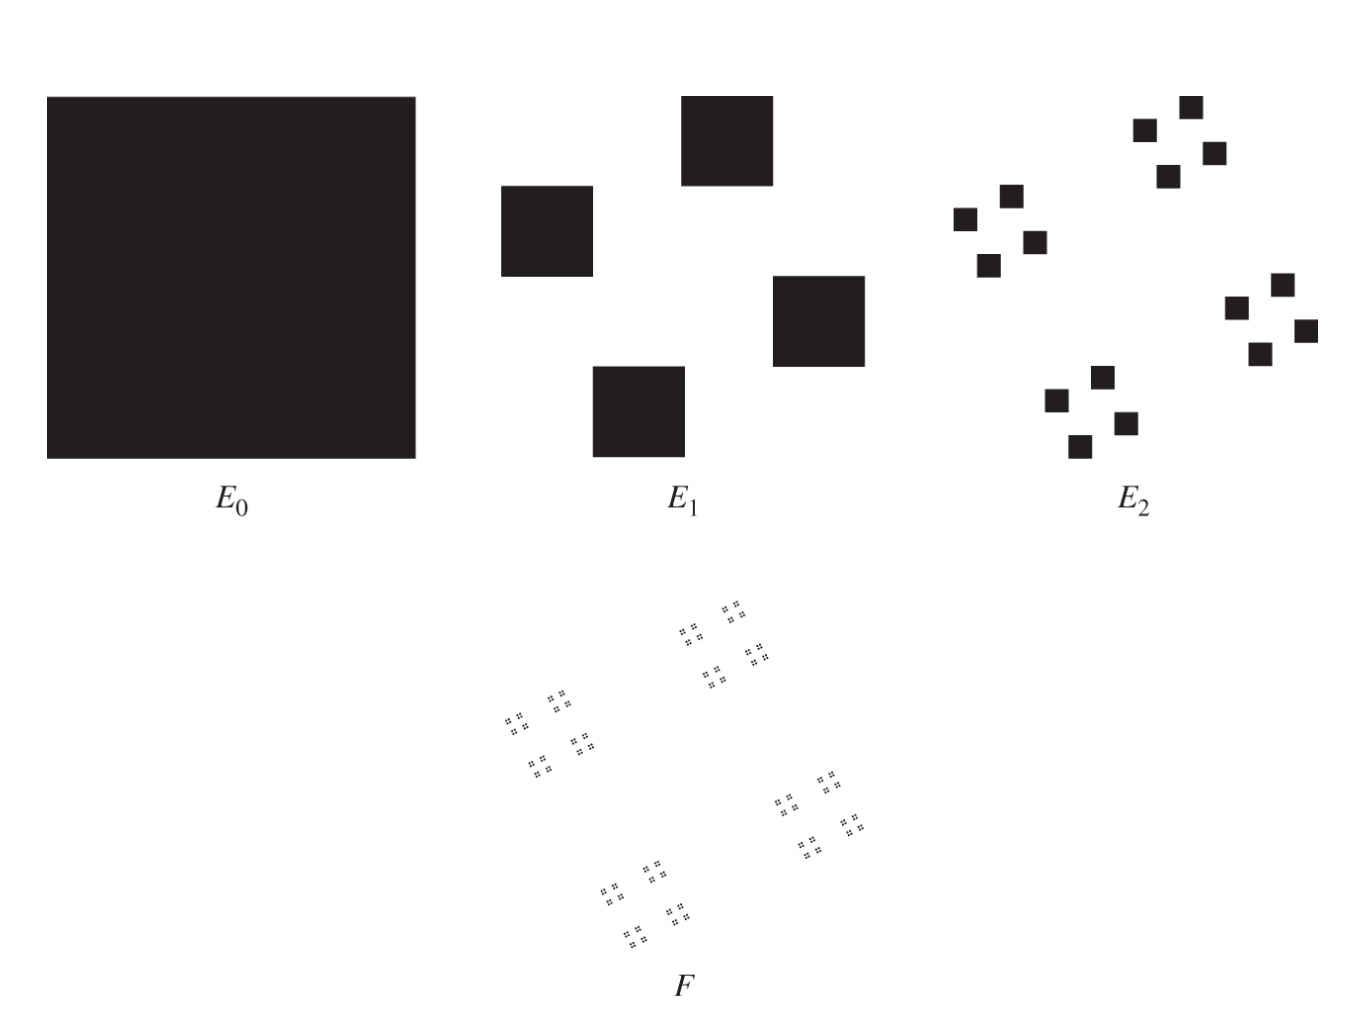
\includegraphics[width=.66\textwidth]{images/cantordust.png}
        \caption{ Construction of a ‘Cantor dust’ }
        \label{fig:cantordust}
    \end{figure}
\end{customexercise}

\begin{customsol}{2.4}
    $k^{\text{th}}$ stage of the construction consists of $4^k$ squares of side length $4^{-k}$. Thus, if $4^{-k} < \delta \leq 4^{-k+1}$, the $4^k$ squares of $E_k$ give a $\delta$ cover of $F$, so $N_\delta(F)\leq 4^k$. Then:
    $$
    \overline{\operatorname{dim}}_{\mathrm{B}} F = \uplim_{\delta\rightarrow 0} \frac{\log N_\delta(F)}{-\log \delta}\leq \uplim_{k\rightarrow\infty} \frac{\log 4^k}{-\log 4^{-k+1}} = 1
    $$
    On the other hand, for $4^{-k-1}\leq \delta < 4^{-k}$, the cube can intersect at most two of the squares of $E_k$. There are $4^k$ squares in $E_k$, all containing points of $F$, so at least $4^k/2$ squares of side $\delta$ are required to cover $F$. Then, $N_\delta (F) \geq 4^{k}/2$, so:
    $$
    \underline{\operatorname{dim}_{\mathrm{B}}} F = \lowlim_{\delta\rightarrow 0}\frac{\log N_\delta(F)}{-\log \delta} \geq \lowlim_{k\rightarrow\infty} \frac{\log 4^k/2}{-\log 4^{-k-1}} = 1
    $$

    Therefore, the box-counting dimension of Cantor dust is 1. 
\end{customsol}



\begin{customexercise}{2.5}
    Use Equivalent definition \ref{bcd-def}(i) to check that the upper box dimension of the von Koch curve(shown in Figure \ref{fig:kochcurve}) is at most $\log 4 / \log 3$ and \ref{bcd-def}(v) to check that the lower box dimension is at least this value.
    \begin{figure}[t]
        \centering
        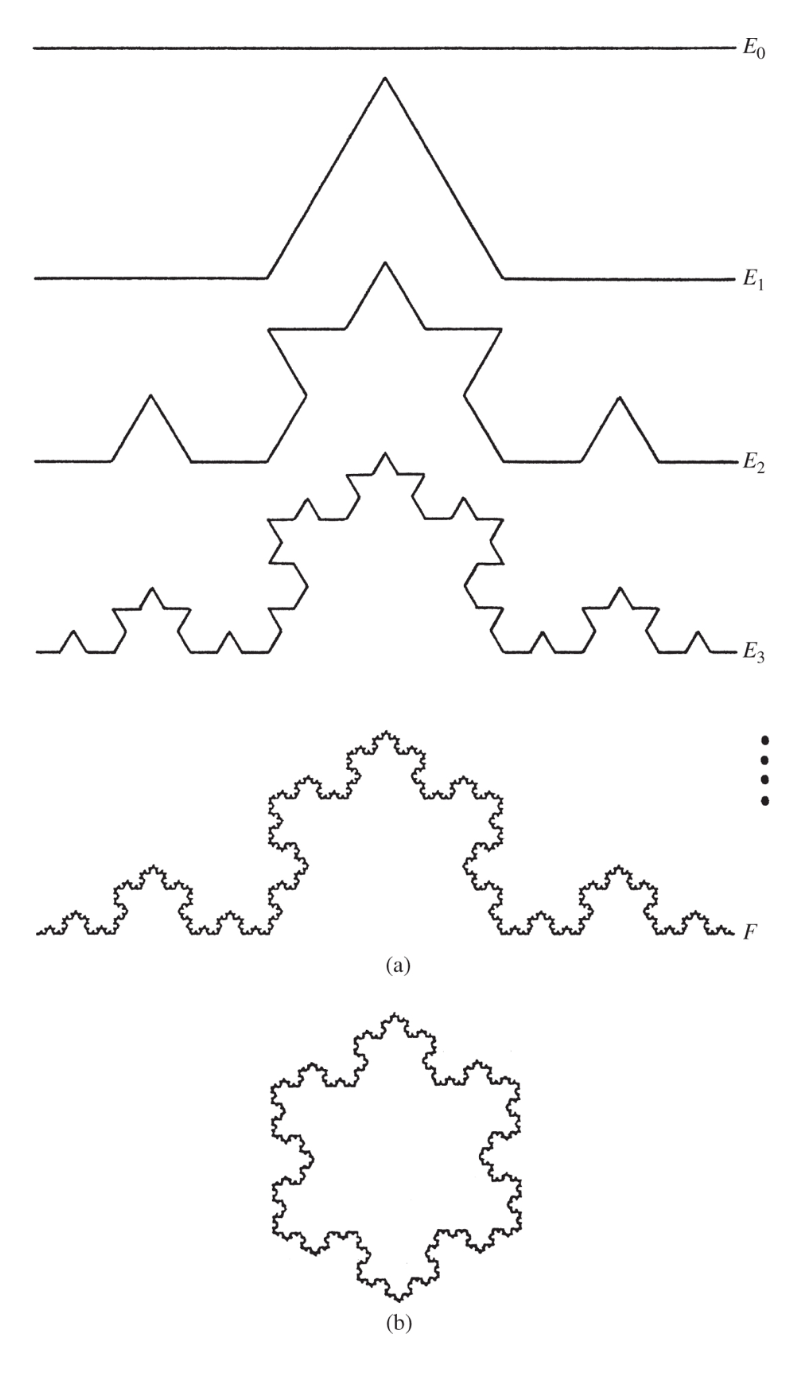
\includegraphics[width=.4\textwidth]{images/Kochcurve.png}
        \caption{(a) Construction of the von Koch curve $F$. At each stage, the middle third of each interval is replaced by the other two sides of an equilateral triangle. (b) Three von Koch curves fitted together to form a snowflake curve.}
        \label{fig:kochcurve}
    \end{figure}
\end{customexercise}

\begin{customsol}{2.5}
    Let $\delta_k = 3^{-k}$, for $E_k$, there are $4^k$ line segments so taking any plane set with diameter at most $\delta_k$ centered at the midpoint of each line segment can cover all points in $F$ so $N_{\delta_k}(F)\leq 4^k$. Then,
    $$
    \overline{\operatorname{dim}}_\mathrm{B}F = \uplim_{k\rightarrow\infty} \frac{\log N_{\delta_k(F)}}{-\log \delta_k}\leq \uplim_{k\rightarrow\infty}\frac{\log 4^k}{\log 3^k} = \frac{\log 4}{\log 3}
    $$
    On the other hand, there are $4^k+1$ vertices of $E_k$ and if we take each vertices as centers of balls with radius $\delta_k = 3^{-k}/2$(it is also sufficient to take $\delta_k = 3^{-k-1}$), there would be at least $4^k+1$ disjoint balls of radius $\delta_k$ with centers in $F$. Then,
    $$
    \begin{aligned}
        \underline{\operatorname{dim}}_{B} F &=\lowlim_{k \rightarrow \infty} \frac{\log N_{\delta_{k}}(F)}{-\log \delta_{k}} \\
        & \geq \lowlim_{k \rightarrow \infty} \frac{\log \left(4^{k}+1\right)}{\log 3^{k+1}} \\
        & \geq \lowlim_{k \rightarrow \infty} \frac{\log \left(4^{k}\right)}{\log 3^{k+1}} \\
        & = \lowlim_{k \rightarrow \infty} \frac{k \log 4}{(k+1) \log 3}\\
        & =\frac{\log 4}{\log 3}
        \end{aligned}
    $$
\end{customsol}




\newpage

\subsection{May 28-31 Measures(1.3)}
\subsubsection{Exercises and Solutions}

\begin{customexercise}{1.18}
    Let $A_{1}, A_{2}, \ldots$ be a decreasing sequence of Borel subsets of $\mathbb{R}^{n}$ and let $A=\bigcap_{k=1}^{\infty} A_{k} .$ If $\mu$ is a measure on $\mathbb{R}^{n}$ with $\mu\left(A_{1}\right)<\infty$, show using (1.6) that $\mu\left(A_{k}\right) \rightarrow \mu(A)$ as $k \rightarrow \infty$.
\end{customexercise}

\begin{customsol}{1.18}
    Consider that $\{A_1\setminus A_k\}$ is an increasing sequence as $\{A_k\}$ decreasing. Then:
    $$ 
    \begin{aligned}
        &\mu\left(\bigcup_{k=1}^{\infty}\left(A_{1}\setminus A_{k}\right)\right) = \mu\left(A_{1} \setminus \bigcap_{k=1}^{\infty} A_{i}\right) = \mu(A_1) - \mu (A) \\
        =&\lim _{k \rightarrow \infty} \mu\left(A_{1} \setminus A_{k}\right) = \lim_{k\rightarrow\infty} (\mu(A_1)-\mu (A_k)) = \mu(A_1) - \lim_{k\rightarrow\infty} \mu(A_k)
    \end{aligned}$$
    As $\mu(A_1)<\infty$, $\displaystyle \lim_{k\rightarrow \infty} \mu(A_k) = \mu(\bigcap_{k=1}^{\infty} A_{i})$
\end{customsol}

\textbf{Conlusion}: For a \textbf{\textit{decreasing sequence}} $A_k$ of Borel subsets of $\mathbb{R}^n$, 
$$\displaystyle \lim_{k\rightarrow \infty} \mu(A_k) = \mu(\bigcap_{k=1}^{\infty} A_{i})$$


\begin{customexercise}{1.23}
    Let $D$ be a Borel subset of $\mathbb{R}^{n}$ and let $\mu$ be a measure 
    on $D$ with $\mu(D)<\infty$. Let $f_{k}: D \rightarrow \mathbb{R}$ be a 
    sequence of functions such that $f_{k}(x) \rightarrow f(x)$ for all $x$ 
    in $D$. Prove \underline{\textbf{Egoroff's theorem}}: that given $\varepsilon>0$ there exists 
    a Borel subset $A$ of $D$ with $\mu(D \backslash A)<\varepsilon$ such that 
    $f_{k}(x)$ converges to $f(x)$ uniformly for $x$ in $A$.
\end{customexercise}

\begin{customsol}{1.23} 
    Assume that for $k, n \in \mathbb{Z}^+$, $A_{k, n} = \{x\in D: |f_l(x) - f(x)| < 1/n, \forall l\geq k\}$(so we consider $\delta = 1/n$ here), 
    then we have $\displaystyle \bigcup_{k=1}^\infty A_{k, n} = D$ and 
    $A_{1, n}\subset A_{2, n}\subset A_{3, n}\subset\dots$. Next, by Property of measure \ref{propmeasure}:
    $$\displaystyle \mu(D) = \mu(\bigcup_{k=1}^\infty A_{k,n}) = \lim_{k\rightarrow\infty}\mu(A_{k,n})<\infty$$
    Hence, 
    $$\displaystyle \lim_{k\rightarrow\infty}\mu(D\setminus A_{k,n}) = \mu(D) - \lim_{k\rightarrow\infty} \mu(A_{k, n}) = 0$$
    Then, $\exists k^\prime \in \mathbb{N}$  s.t. whenever 
    $k\geq k^\prime$, $\mu(D\setminus A_{k,n}) < \displaystyle \frac{\epsilon}{2^n}$. 
    Next, we can construct $\displaystyle A = \bigcap_{n = 1}^\infty A_{k',n}$, which is a Borel subset of $D$ and satisfies:
    $$\mu(D\setminus A) = \mu(D\setminus \bigcap_{n=1}^\infty A_{k', n}) = \mu(\bigcup_{n=1}^\infty D\setminus A_{k',n}) = \sum_{n=1}^\infty \mu(D\setminus A_{k',n}) < \sum_{n=1}^\infty \frac{\epsilon}{2^n} = \epsilon$$
    As $\displaystyle \sum_{n=1}^{\infty} \frac{1}{2^n} = 1$, and $A$ exists for the question. 
    Finally, $\forall\delta > 0, n > 1/\delta, \forall x\in A$ where $x\in A_{k', n}$ as well, such that whenever $k\in\mathbb{N}, k>k'$, $|f_k(x) - f(x)| < 1/n < \delta\Rightarrow$ $f_k(x)$ converges to $f(x)$ uniformly for $x$ in $A$.
    
    \end{customsol}

\textbf{Note: }$\displaystyle \sum_{n=1}^{\infty} \frac{1}{2^n} = 1$ is always used to construct $\epsilon$ in analysis proofs.
 
\begin{customexercise}{1.24}
    Prove that if $\mu$ is a measure on $D$ and $f: D \rightarrow \mathbb{R}$ satisfies $f(x) \geq 0$ for all $x$ in $D$ and $\int_{D} f \mathrm{~d} \mu=0$ then $f(x)=0$ for $\mu$ -almost all $x$.
\end{customexercise}

\begin{customsol}{1.24}
Suppose $f(x)\geq\epsilon>0$ on a set $E_\epsilon\subset D$ given $\epsilon>0$, we have for $x\in D\setminus E_\epsilon, f(x)=0$ and then:
$$\begin{aligned}
    0 &= \int_D f(x) d\mu\\ &= \int_{E_\epsilon} f(x)d\mu + \int_{D\setminus E_\epsilon} f(x)d\mu\\
    &\text{As }\epsilon \chi_{E_\epsilon}(x) \text{ is a simple function and by the integral of more general functions}\\
    &\geq \int \epsilon \chi_{E_\epsilon}(x) d\mu + 0 \\ &= \epsilon\mu(E_\epsilon) + 0
\end{aligned}$$
As $\epsilon\mu(E_\mu)\leq 0$ while $\epsilon>0$, we have $\mu(E_\epsilon) = 0 \Rightarrow \mu\left(\bigcup_{\epsilon\in\mathbb{R}^+} E_\epsilon\right) = \mu\left(\{x: f(x)>0\}\right) = 0\Rightarrow f(x) = 0$ for $\mu$-a.e.. 
\end{customsol}

\textbf{Note: } 
\begin{enumerate}
    \item $f(x) = 0$ for $\mu-$a.e $\Leftrightarrow$ The set of points where $f(x)!=0$($f(x)>0$ in this case) has measure zero.
    \item $\displaystyle\int_E 1 d\mu = \mu(E)$
\end{enumerate}
\begin{definition}[Simple Function]
    Simple functions are sums of linear combination of characteristic functions, e.g. $\displaystyle f(x) = \sum a_i \chi_{A_i}(x)$
\end{definition}

\newpage

\subsection{May 26 Functions and Limits(1.2)}
\subsubsection{Exercises and Solutions}
\begin{customexercise}{1.12}
    Let $f, g:[0,1] \rightarrow \mathbb{R}$ be Lipschitz functions. 
    Show that the functions defined on $[0,1]$ by $f(x)+g(x)$ and 
    $f(x) g(x)$ are also Lipschitz.
\end{customexercise}

\textbf{Solution}:  
\begin{enumerate}[(i)]
    \item As $f, g$ are Lipschitz function, we have $|f(x)-f(y)| \leq c_1|x-y|$ and $|g(x)-g(y)| \leq c_2|x-y|$  where $\forall x, y \in [0, 1]$ and $c_1, c_2 \geq 0$.
    Then, $|(f(x)+g(x)) - (f(y) + g(y))| = |f(x) - f(y) +g(x) - g(y)| \leq  |f(x) - f(y)| + |g(x) - g(y)|\leq (c_1 + c_2 )\cdot |x - y|, \forall x, y\in[0, 1] $. Since $(c_1+c_2)\geq 0$, the condition is satisfied and therefore
    the functions defined on $[0,1]$ by $f(x)+g(x)$ is Lipschitz. 
    \item Consider that $|f(x) -f(0)| \leq c_1 |x| \leq c_1, x\in[0, 1]$, so we have non-negative $c_3 = |f(0)| + c_1 \geq |f(x)|$. Similarly, 
    we have non-negative $c_4 \geq |g(x)|$
    
    $|f|, |g| < 1$, $\forall x, y\in[0, 1]$\\
    $\begin{aligned}
        &|f(x)g(x) - f(y)g(y)| \\
        =& |f(x)g(x) -f(x)g(y) + f(x)g(y)- f(y)g(y)| \\
        =& |f(x)(g(x) - g(y)) + g(y)(f(x) - f(y))| \\ 
        \leq& |g(y)||(f(x) - f(y))| + |f(x)||(g(x) - g(y))| \\
        \leq& c_1 c_4 ||x-y| + c_2 c_3|x-y| \\
        \leq& (c_1c_4 +c_2c_3) |x-y|
    \end{aligned}$\\
    Since $c_1c_4 +c_2c_3 \geq 0$, the condition is satisfied and therefore
    the functions defined on $[0,1]$ by $f(x)g(x)$ is Lipschitz.
\end{enumerate}


\begin{customexercise}{1.13(Rademacher's theorem)}\label{1.13}
    Let $f: \mathbb{R} \rightarrow \mathbb{R}$ be differentiable 
    with $\left|f^{\prime}(x)\right| \leq c$ for all $x$. 
    Show, using the mean value theorem, that $f$ is a Lipschitz function.
\end{customexercise}

\textbf{Solution}: 
$\forall x, y \in \mathbf{R} , x \neq y$, by mean-value theorem, $\exists w \in(x, y)$ such that 
$$
\begin{aligned}
    &\frac{f(y)-f(x)}{y-x}=f^{\prime}(w) \\
    \Rightarrow  &\left|\frac{f(y)-f(x)}{y-x}\right|=\left|f^{\prime}(w)\right| \leq c \\
    \Rightarrow &|f(x)-f(y)| \leq c|x-y| \quad (x, y \in \mathbb{R})
\end{aligned}
$$

Therefore, $f$ is a Lipschitz function.


\begin{customexercise}{1.14}
    Show that every Lipschitz function 
    $f: \mathbb{R} \rightarrow \mathbb{R}$ is continuous.
\end{customexercise}

\textbf{Solution: } See proof wrote for Theorem \ref{LipschitzContinuous}.


\begin{customexercise}{1.15}
    Let $f: \mathbb{R} \rightarrow \mathbb{R}$ be given by $f(x)=x^{2}+x .$ 
    Find (i) $f^{-1}(2)$, (ii) $f^{-1}(-2)$ and (iii) $f^{-1}([2,6])$.
\end{customexercise}

\textbf{Solution}: As $f(x) = x^2 + x$, $\displaystyle x = -\frac{1}{2} \pm \frac{\sqrt{1 + 4y}}{2}$
\begin{enumerate}[(i)]
    \item $f^{-1}(2) = \{-2, 1\}$
    \item $f^{-1}(-2) = \emptyset$
    \item As $\displaystyle x = -\frac{1}{2} + \frac{\sqrt{1 + 4y}}{2}$ is increasing and $\displaystyle x = -\frac{1}{2} - \frac{\sqrt{1 + 4y}}{2}$ is decreasing while y increasing, 
     $f^{-1}([2,6]) = [-3, -2]\cup [1, 2]$
\end{enumerate}


\begin{customexercise}{1.16}
    Show that $f(x)=x^{2}$ is Lipschitz on $[0,2]$, bi-Lipschitz on 
    $[1,2]$ and not Lipschitz on $\mathbb{R}$.
\end{customexercise}

\textbf{Solution}: 
\begin{enumerate}[(i)]
    \item As $\forall x, y\in [0,2]$, $|x+y|\leq 4$, we have $|f(x)-f(y)|=\left|x^{2}-y^{2}\right|=|x+y||x-y| \leq 4|x-y|$.
    Thus, $f$ is Lipschitz on $[0,2]$.
    \item Apparently, $2|x-y|\leq|f(x) - f(y)|\leq 4|x-y|$ by above. As $f([1, 2]) = [1, 4]$, $\forall x, y \in [1, 4]$, $\displaystyle \frac{1}{\sqrt{x}+\sqrt{y}} \leq \frac{1}{2}$, we have: \\
    \(
    \begin{aligned}
        &\displaystyle \left|f^{-1}(x)-f^{-1}(y)\right|=|\sqrt{x}-\sqrt{y}|=\left|\frac{x-y}{\sqrt{x}+\sqrt{y}}\right| \leq \frac{1}{2}|x-y|\\
        \Rightarrow & \text{ so } f^{-1} \text{ is Lipschitz on } [1,4]. \\
        \Rightarrow & f \text{ is bi-Lipschitz on }[1,2].
    \end{aligned}
    \)
    \item Let $x = ky, k\in\mathbb{R}\setminus\{0\}$, then $\displaystyle \frac{|f(x) - f(y)|}{|x - y|} = \frac{|k^2y^2 - y^2|}{|ky - y|} = \left|\frac{k^2 - 1}{k-1} \right | |y|$, which is unbounded on $\mathbb{R}$. Therefore, the Lipschitz constant does not exist and $f$ is not Lipschitz on $\mathbb{R}$

\end{enumerate}


\newpage
